\chapter{Graphical User Interfaces}
\label{chap:windows}

A \idx{command-line interface} (\idx{CLI}) is a method for communicating with the user through text. In contrast, a \idx{graphical user interface} (\idx{GUI}) extends the ways of communicating with the user to also include organising the screen space in windows, icons, and other visual elements, and a typical way to activate these elements are through a pointing device such as the mouse or by touch. Some of these elements may themselves be textual, and thus most operating systems offers access to a command-line interface in a window alongside other interface types.

Fsharp includes a number of implementations of graphical user interfaces, but at time of writing only \idx{WinForms} is supported on both the Microsoft .Net and the Mono platform, and hence, WinForms will be the subject of the following chapter.

WinForms is designed for \idx{event driven programs}, which spends most time waiting for the user to perform an action, called and event, and for each event has a set of predefined responses to be performed by the program. For example, Figure~\ref{fig:safariGui} shows the program Safari, which is a graphical user interface for accessing web-servers.
\begin{figure}
  \centering
  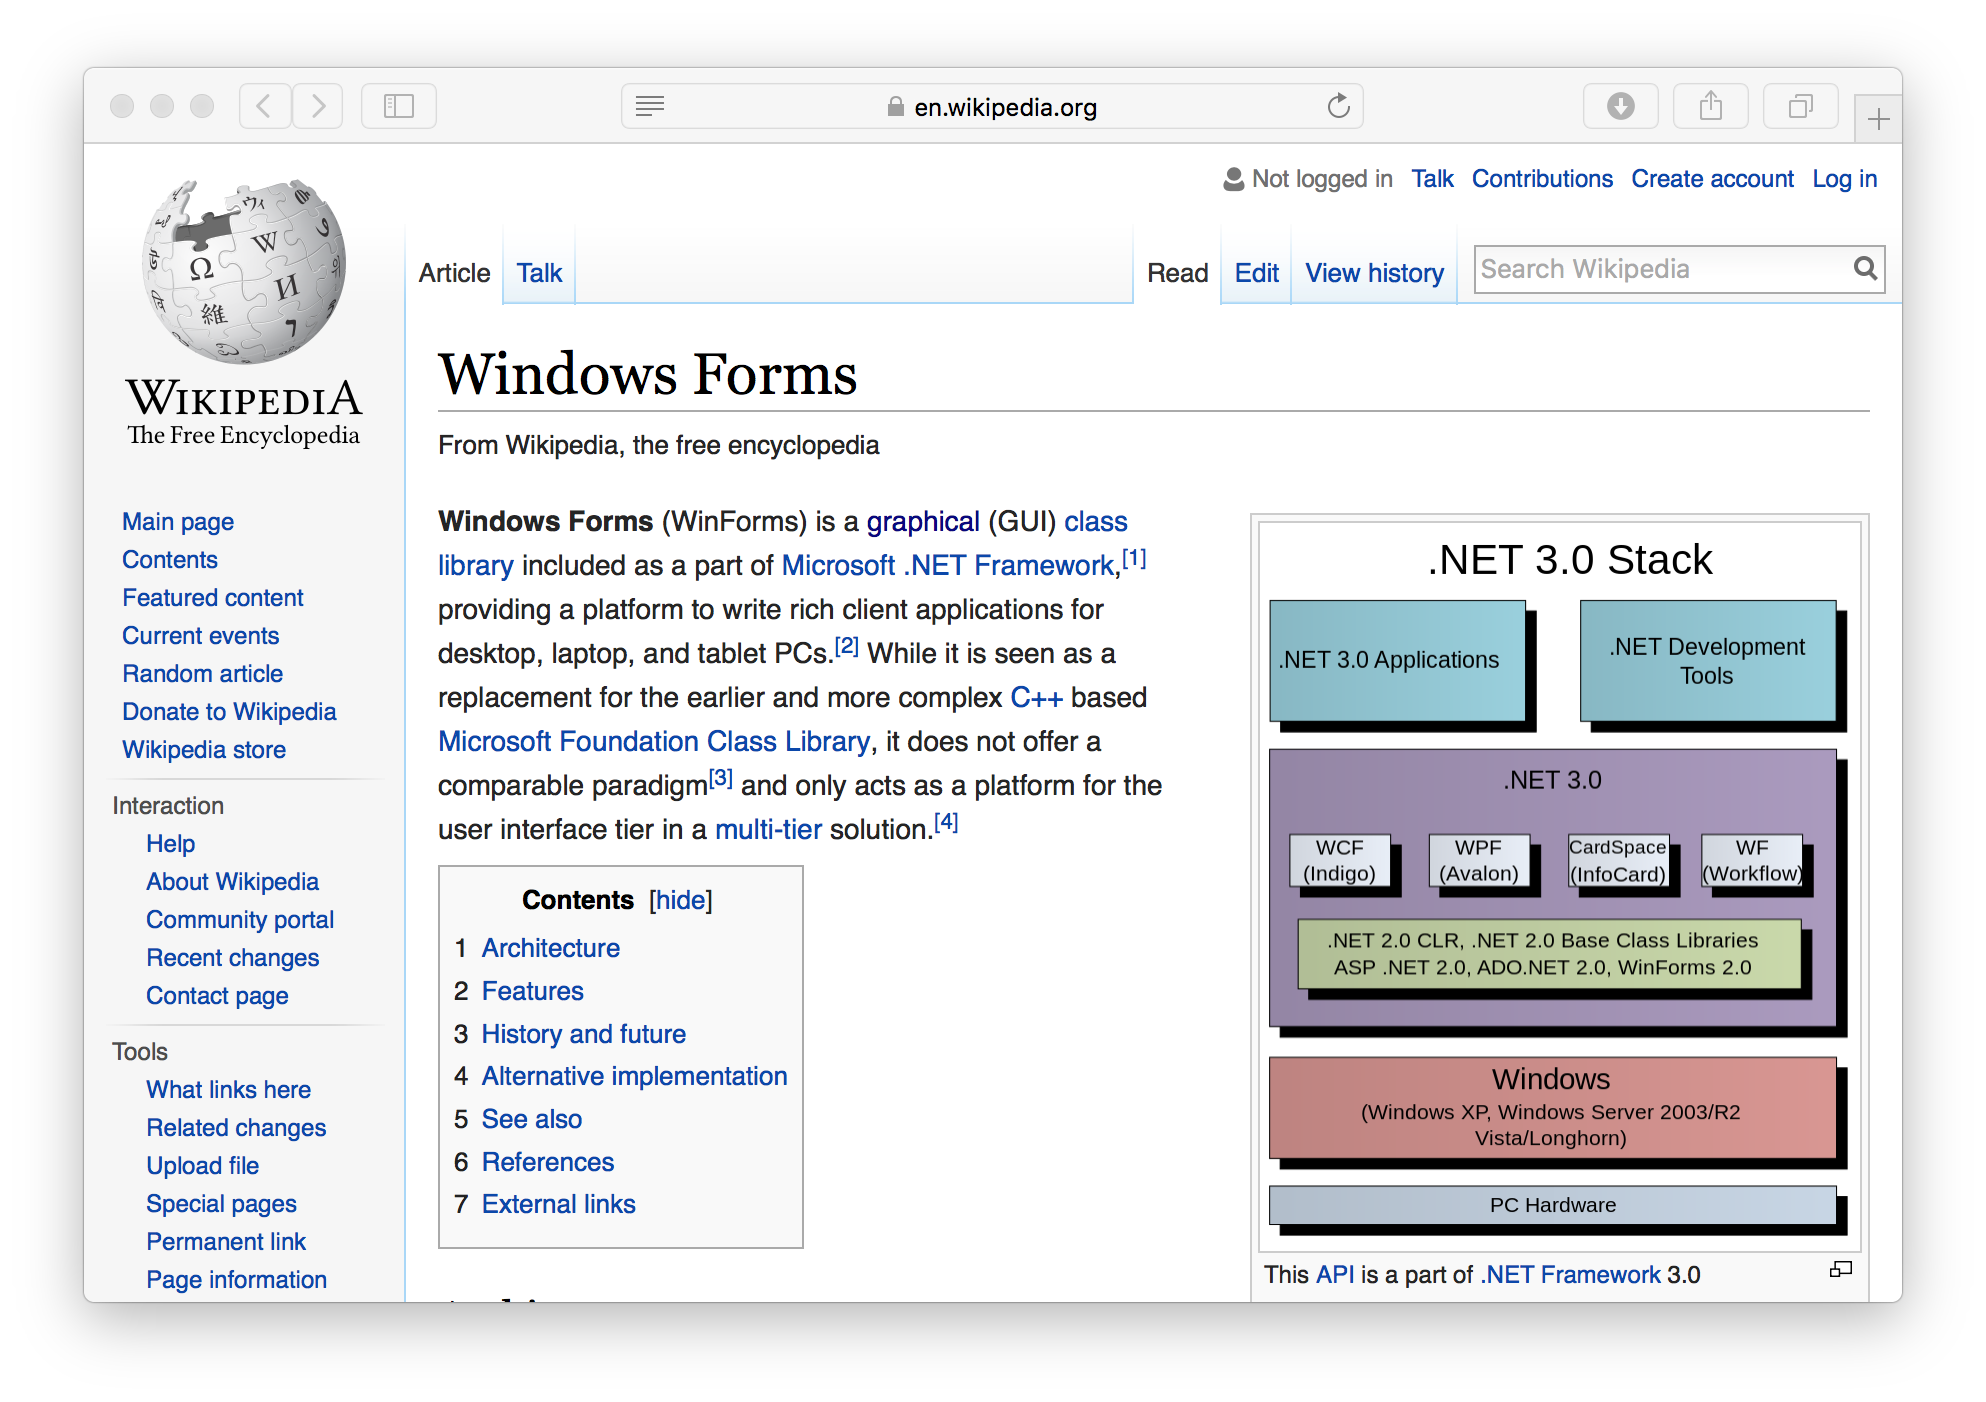
\includegraphics[width=0.6\textwidth]{safariWinForms}
  \caption{A web-browser is a graphical user interface for accessing a web-server and interacting with its services. Here the browser is showing the page \url{https://en.wikipedia.org/wiki/Windows_Forms} at time of writing.}
  \label{fig:safariGui}
\end{figure}
The program present information to the user in terms of text and images, and has areas that when activated by clicking with a mouse or similar allows the user to, e.g., go to other web-pages by type URL, to follow hyperlinks, and to generate new pages by entering search queries.

\section{Drawing primitives in Windows}
WinForms is based on two namespaces: \lstinline!System.Windows.Forms! and \lstinline!System.Drawing!. To start making a graphical display on the screen, the first thing to do is open a window, which acts as a reserved screen space for our output. With WinForms, this may be done as shown in Listing~\ref{winforms/openWindow}, and the result is shown in Figure~\ref{fig:openWindow}.
%
\fsCode{winforms/openWindow}{Create the window and turn over control to the operating system.}
%
\begin{figure}
  \centering
  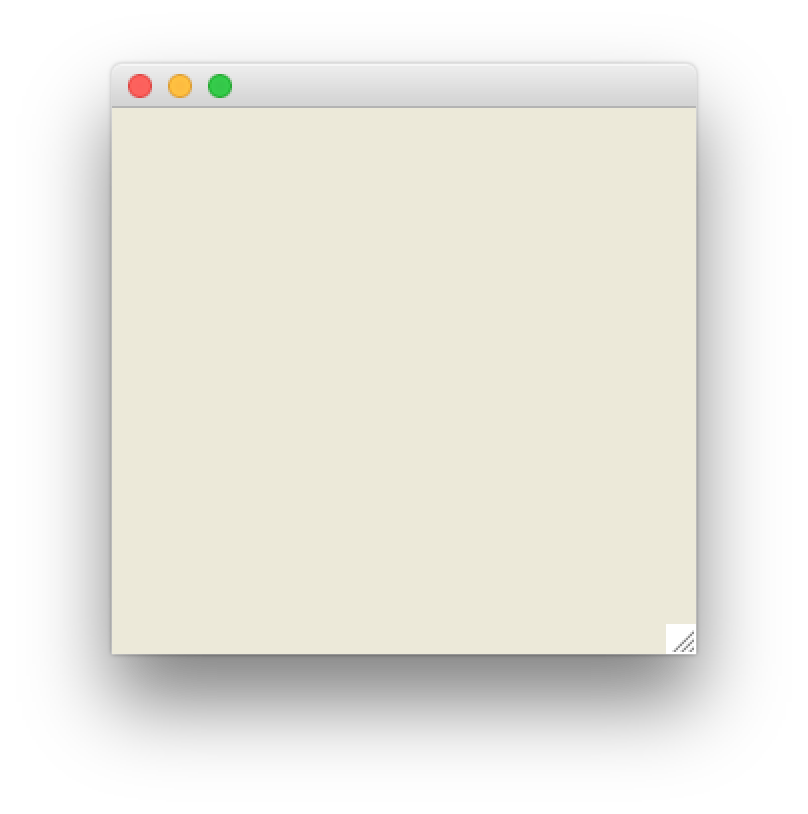
\includegraphics[width=0.6\textwidth]{openWindow}
  \caption{A window opened by Listing~\ref{winforms/openWindow}.}
  \label{fig:openWindow}
\end{figure}
The \lstinline!new System.Windows.Forms.Form ()! creates an object (See Chapter~\ref{chap:oop}), but does not display the window on the screen. When the function \lstinline!System.Windows.Forms.Application.Run! is applied to the object, then the control is handed over to the WinForm's \idx{event-loop}, which continues until the window is closed by, e.g., pressing the icon designated by the operating system. On the mac OSX that is the red button in the top left corner of the window frame, and on Window it is the cross on the top right corner of the window frame.

The window, which WinForms calls a form, has a long list of \idx{methods} and \idx{properties}. E.g., the background color may be set by \lstinline!BackColor!, the title of the window may be set by \lstinline!Text!, and you may get and set the size of the window with the \lstinline!Size!. This is demonstrated in Listing
%
\fsCode{winforms/windowAttributes}{Create the window and changing its properties.}
%
\begin{figure}
  \centering
  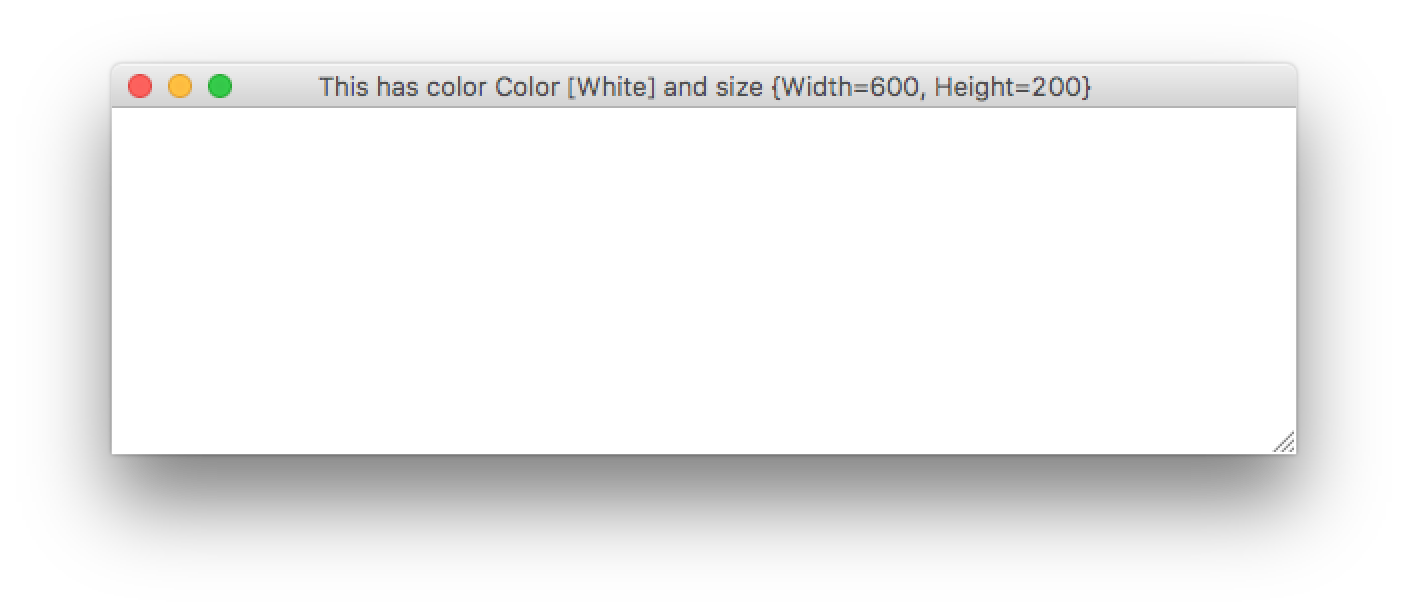
\includegraphics[width=0.6\textwidth]{windowAttributes}
  \caption{A window with user-specified size and background color, see Listing~\ref{winforms/windowAttributes}.}
  \label{fig:openWindow}
\end{figure}
These properties have been programmed as \idx{accessors} implying that they may used as mutable variables. The \idx{\lstinline{System.Drawing.Color}} is a general structure for specifying colors as 4 channels: alpha, red, green, blue, where each channel is an 8 bit unsigned integer, where the alpha channel specifies the transparency of a color, where values 0--255 denotes the range of fully transparent to fully opaque, and the remaining channels denote the amount of red, green, and blue where 0 is none and 255 is full intensity. Any color may be created using the \lstinline!FromArgb! method, e.g., an opaque red is given by \lstinline!System.Drawing.Color.FromArgb (255, 255, 0, 0)!. There are also many build-in colors, e.g., the same red color is also a known color and may be obtained as \lstinline!System.Drawing.Color.Red!. For a given color, then the 4 alpha, red, green, and blue channel's values may be obtained as the \lstinline!A!, \lstinline!R!, \lstinline!G!, \lstinline!B!, see Listing~\ref{drawingColors}
%
\fs{drawingColors}{Defining colors and accessing their values.}
%
The \lstinline!System.Drawing.Size! is a general structure for specifying sizes as height and width pair of integers.

WinForms supports drawing of simple graphics primitives. Simple examples are \lstinline!System.Drawing.Pen! to specify the color to be drawn, \lstinline!System.Drawing.Point! to specify a pair of coordinates, and \lstinline!System.Drawing.Graphics.DrawLine!. \lstinline!DrawLine! is different than the previous examples since it must be related to a specific device, and it is typically accessed as an event. Displaying graphics in WinForms is performed as the reaction to an event. E.g., windows are created by the program, moved, minimized, occluded by other windows, resized, etc., by the user or the program, and each action may require that the content of the window is refreshed. Thus, we must create a function that WinForms can call, when it determines that the content needs to be redrawn. This is known as a \idx{call-back function}, and it is added to an existing form using the \lstinline!Paint.Add! function. As an example, consider the problem of draw a triangle in a window. For this we need to make a function that can draw a triangle not once, but any time WinForms determines it necessary to draw and redraw the triangle. Drawing is done with reference to a coordinate system. WinForms operates with several coordinate systems, the most important is the \idx{screen coordinates}. Screen coordinate $(x,y)$ have their origin in the top-left corner, and $x$ increases to the right, while $y$ increases down.\jon{Possibly something about client coordinates and world coordinates.} Thus, we may draw a triangle as demonstrated in Listing~\ref{winforms/triangle}.
%
\fsCode{winforms/triangle}{Adding line graphics to a window.}
%
\begin{figure}
  \centering
  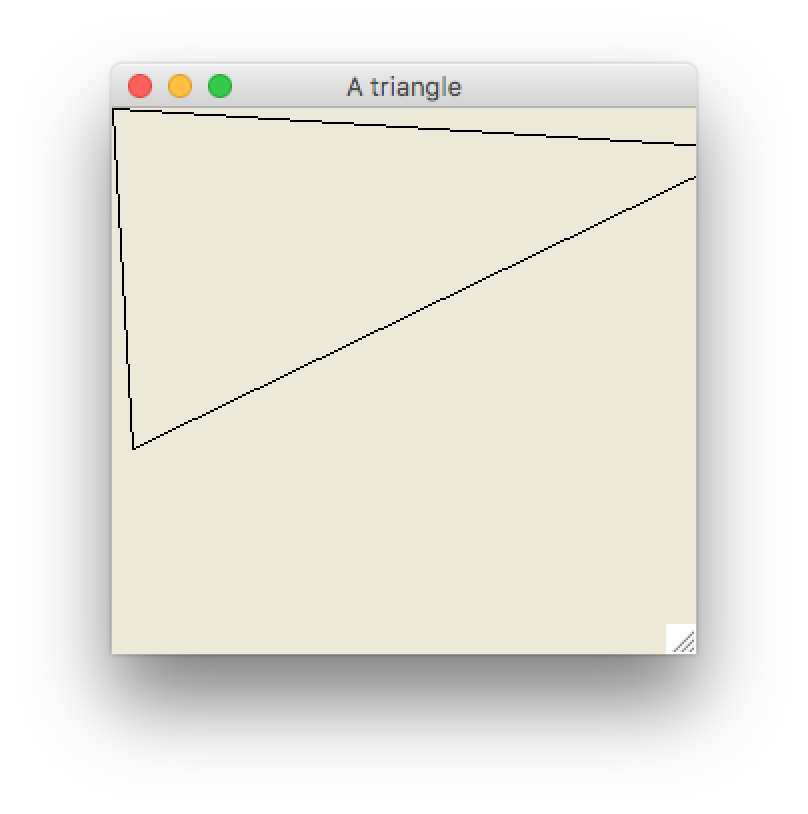
\includegraphics[width=0.6\textwidth]{triangle}
  \caption{Drawing a triangle using Listing~\ref{winforms/triangle}.}
  \label{fig:triangle}
\end{figure}
A walk-through of the code is as follows: First we create an array of points and a pen color, then we create a pen and a window. The method for drawing the triangle is added as an anonymous function using the created window's \lstinline!Paint.Add! method. This function is to be called as a response to a paint event, and takes a \lstinline!PaintEventArgs! object, which includes the System.Drawing.Graphics object. Since this object will be related to a specific device, when \lstinline!Paint! is called then we may call the \lstinline!DrawLine! function to sequentially draw lines between our array of points. Finally, we hand the form to the event-loop, which as one of the earliest events will open the window and call the \lstinline!Paint! function we have associated with the form.

%
\fsCode{winforms/triangleOrganized}{Improved organization of code for
  drawing a triangle. Compare with Listing~\ref{winforms/triangle}.}
%
\begin{figure}
  \centering
  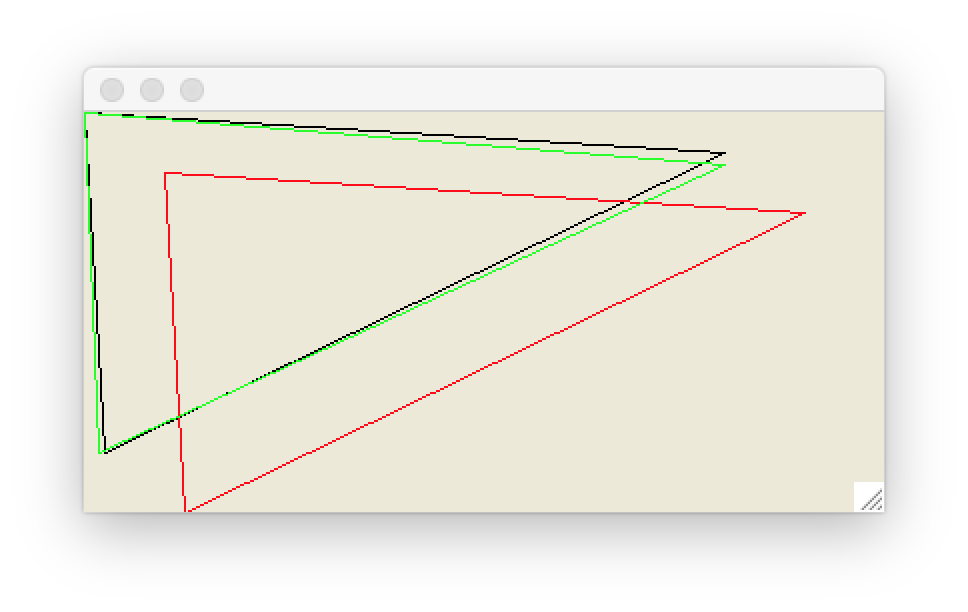
\includegraphics[width=0.6\textwidth]{triangleOrganized}
  \caption{Better organization of the code for drawing a triangle, see Listing~\ref{winforms/triangleOrganized}.}
  \label{fig:triangleOrganized}
\end{figure}
\jon{requires the introduction of type declarations.}\jon{Remember to talk about pen width.}

%
\fsCode[numbers=left,numbersep=6pt,numberstyle=\scriptsize\color{white},lastline=42]{winforms/transformWindows}{Reusable
  code for drawing in windows.}
\fsCode[numbers=left,numbersep=6pt,numberstyle=\scriptsize\color{white},firstnumber=44,firstline=44]{winforms/transformWindows}{Code for drawing triangles using the reusable part shown in Listing~\ref{winforms/transformWindows}.}
%
\begin{figure}
  \centering
  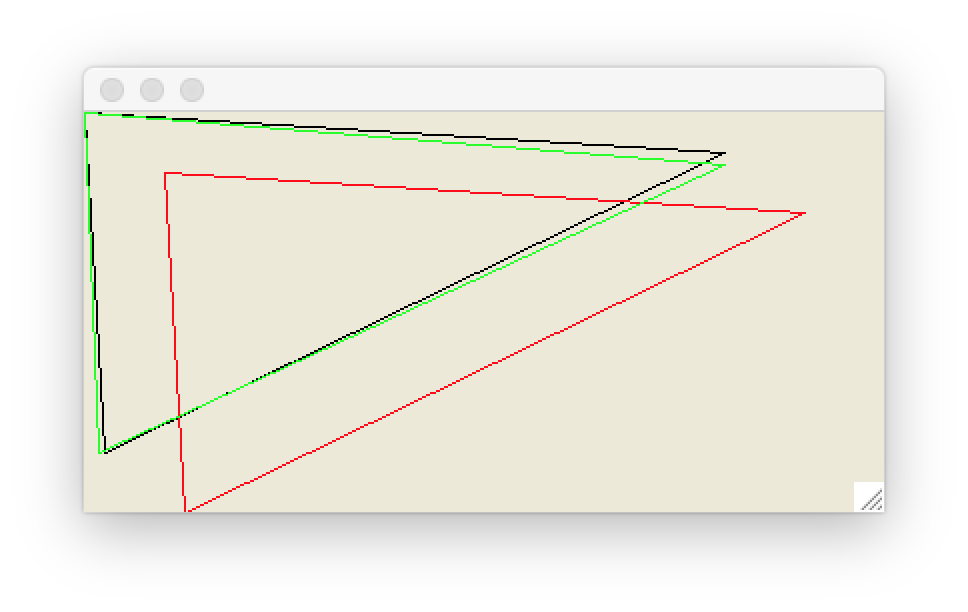
\includegraphics[width=0.6\textwidth]{transformWindows}
  \caption{Transformed versions of the same triangle resulting from running the code in Listing~\ref{winforms/transformWindows}.}
  \label{fig:transformWindow}
\end{figure}

\begin{problem}
  Given a triangle produce a Mandela drawing, where $n$ rotated versions of the triangle is drawn around its center of mass.
\end{problem}
%
\fsCode[numbers=left,numbersep=6pt,numberstyle=\scriptsize\color{white},firstnumber=44,firstline=44]{winforms/rotationalSymmetry}{Create the window and changing its properties.}
%
\begin{figure}
  \centering
  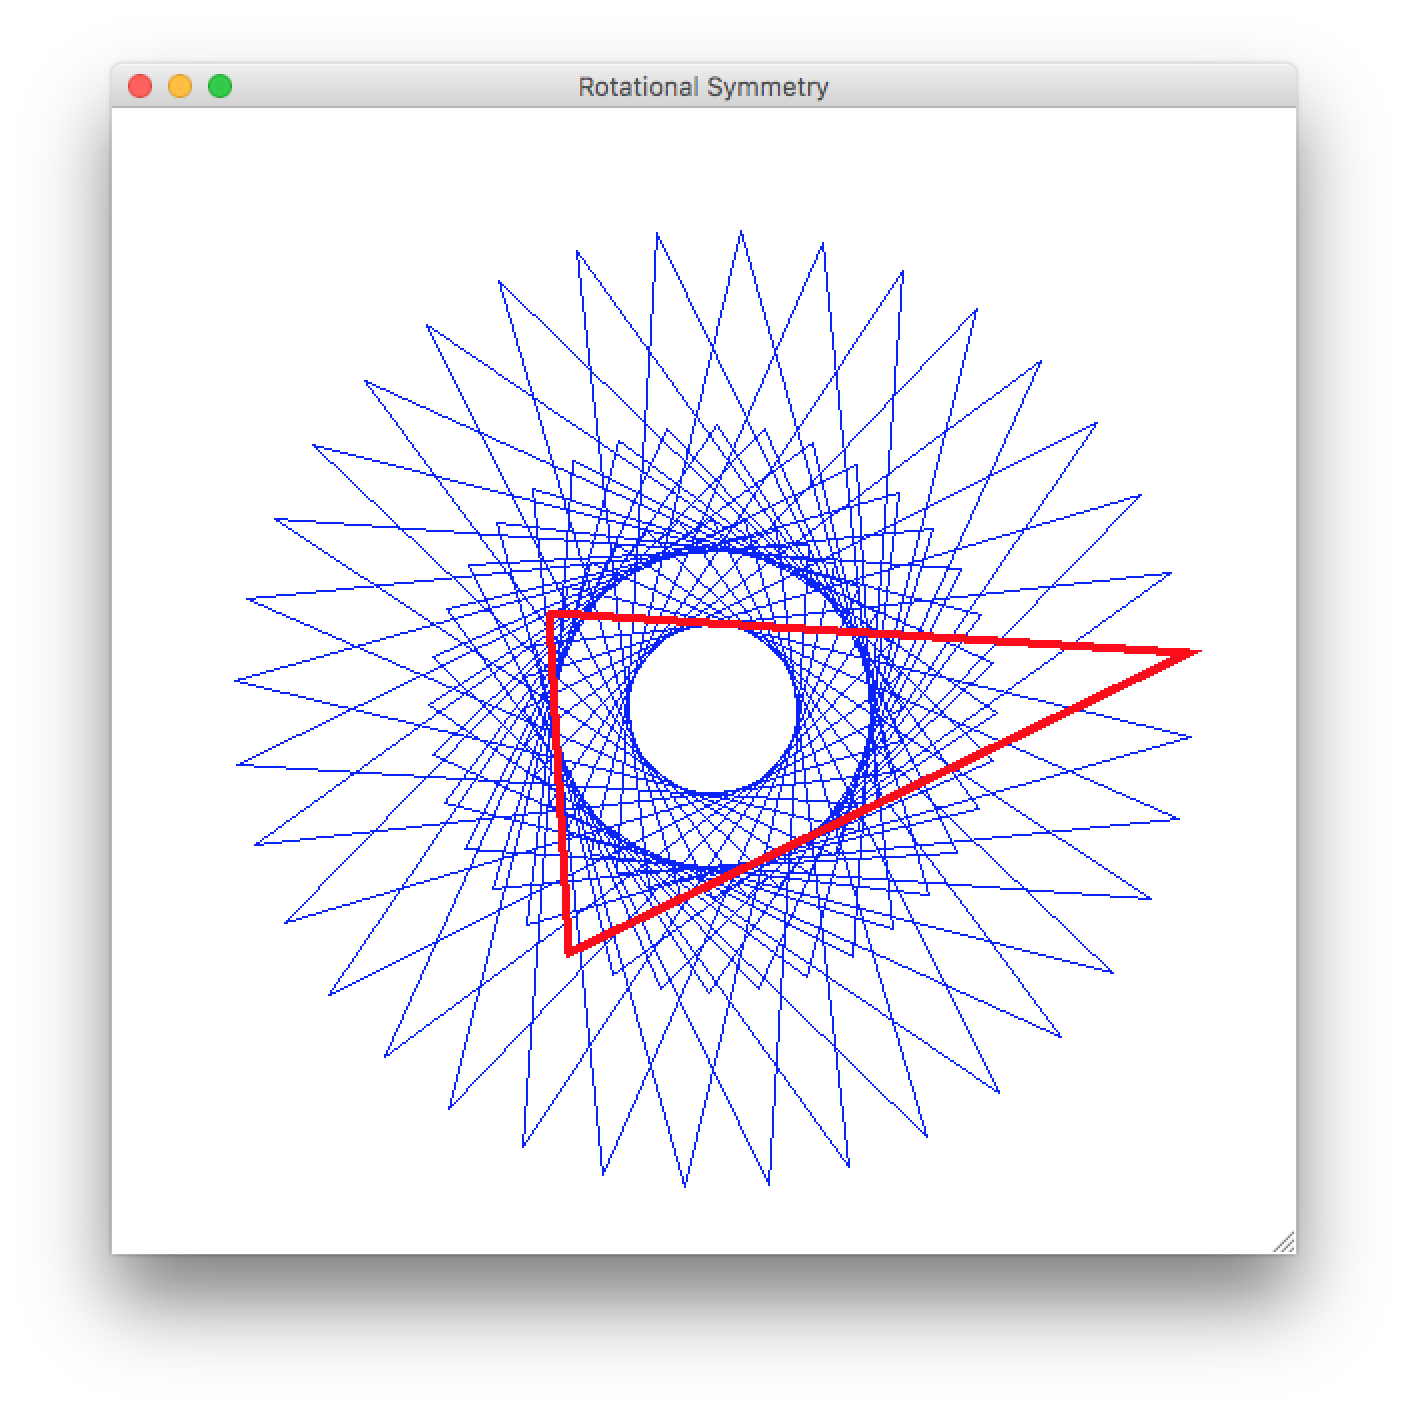
\includegraphics[width=0.8\textwidth]{rotationalSymmetry}
  \caption{A symmetric figure resulting from Listing~\ref{winforms/rotationalSymmetry}.}
  \label{fig:rotationalSymmetry}
\end{figure}

\jon{Add other things to draw: filled stuff, clearing, circles, text}

\begin{table}
  \begin{center}
  \rowcolors{2}{oddRowColor}{evenRowColor}
    \begin{tabularx}{\linewidth}{|l|X|}
      \hline
      \rowcolor{headerRowColor}  Function & Description\\
      \hline
      \lstinline{DrawArc : Pen * Rectangle * Single * Single}
      &Draws an arc representing a portion of an ellipse specified by a Rectangle structure.\\
      \hline
      \lstinline{DrawBezier : Pen * Point * Point * Point * Point}	
      &Draws a Bézier spline defined by four Point structures.\\
      \hline
      \lstinline{DrawClosedCurve : Pen * Point[]}	
      &Draws a closed cardinal spline defined by an array of Point structures.\\
      \hline
      \lstinline{DrawCurve : Pen * Point[]}	
      &Draws a cardinal spline through a specified array of Point structures.\\
      \hline
      \lstinline{DrawEllipse : Pen * Rectangle}	
      &Draws an ellipse specified by a bounding Rectangle structure.\\
      \hline
      \lstinline{DrawImage : Image * Point[]}	
      &Draws the specified Image at the specified location and with the specified shape and size.\\
      \hline
      \lstinline{DrawLines : Pen * Point[]}	
      &Draws a series of line segments that connect an array of Point structures.\\
      \hline
      \lstinline{DrawPie : Pen * Rectangle * Single * Single}	
      &Draws a pie shape defined by an ellipse specified by a Rectangle structure and two radial lines.\\
      \hline
      \lstinline{DrawPolygon : Pen * Point[]}	
      &Draws a polygon defined by an array of Point structures.\\
      \hline
      \lstinline{DrawRectangles : Pen * Rectangle[]}	
      &Draws a series of rectangles specified by Rectangle structures.\\
      \hline
      \lstinline{DrawString : String * Font * Brush * PointF}	
      &Draws the specified text string at the specified location with the specified Brush and Font objects.\\
      \hline
      \lstinline{FillClosedCurve : Brush * Point[]}	
      &Fills the interior of a closed cardinal spline curve defined by an array of Point structures.\\
      \hline
      \lstinline{FillEllipse : Brush * Rectangle}	
      &Fills the interior of an ellipse defined by a bounding rectangle specified by a Rectangle structure.\\
      \hline
      \lstinline{FillPie : Brush * Rectangle * Single * Single}	
      &Fills the interior of a pie section defined by an ellipse specified by a RectangleF structure and two radial lines.\\
      \hline
      \lstinline{FillPolygon : Brush * Point[]}	
      &Fills the interior of a polygon defined by an array of points specified by Point structures.\\
      \hline
      \lstinline{FillRectangle : Brush * Rectangle}	
      &Fills the interior of a rectangle specified by a Rectangle structure.\\
      \hline
      \lstinline{FillRegion : Brush * Region}	
      &Fills the interior of a Region.\\
      \hline
    \end{tabularx}
  \end{center}
  \caption{Some methods of the \lstinline!System.IO.Path! class.}
  \label{tab:path}
\end{table}

\section{Programming intermezzo}
\begin{problem}
  Consider a curve consisting of piecewise straight lines all with the same length but with varying angles $0^{\circ}$, $90^{\circ}$, $180^{\circ}$, or $270^{\circ}$ w.r.t.\ the horisontal axis. To draw this curve we need 3 basic operations: Draw ($F$), turn right ($+$), and turn left ($-$). The turning is w.r.t.\ the present diretion. A Hilbert Curve is a spacefilling curve, which be expressed recursively as:
\begin{align}
  A &\rightarrow -BF+AFA+FB-\label{eq:hilbertA}\\
  B &\rightarrow +AF-BFB-FA+\label{eq:hilbertB}
\end{align}
starting with $A$. The order of the curve is the depth of the recursion, and to draw a 0'th order curve, we don't recurse at all, i.e., ignore all occurrences of the symbols $A$ and $B$ on the right-hand-side of \eqref{eq:hilbertA}, and get $-F+F+F-$. For the 1'st order curve, we recurse once, i.e., 
\begin{align*}
  A 
  \rightarrow &-BF+AFA+FB- \\
  \rightarrow &-(+AF-BFB-FA+)F\\
               &\quad+(-BF+AFA+FB-)F(-BF+AFA+FB-)\\
               &\qquad +F(+AF-BFB-FA+)-\\
  \rightarrow &AF-BFB-FA+FBF+AFA+FB-F-BF+AFA+FBF+AF-BFB-FA\\
  \rightarrow &F-F-F+FF+F+F-F-F+F+FF+F-F-F
\end{align*}
Make a program, that given an order produces an image of the Hilbert curve.
\end{problem}
%
\fsCode[numbers=left,numbersep=6pt,numberstyle=\scriptsize\color{white},firstnumber=44,firstline=44]{winforms/hilbert}{Create the window and changing its properties.}
%
\begin{figure}
  \centering
  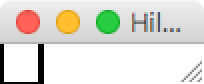
\includegraphics[width=0.45\textwidth]{hilbert1}
  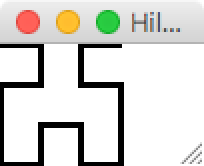
\includegraphics[width=0.45\textwidth]{hilbert2}
  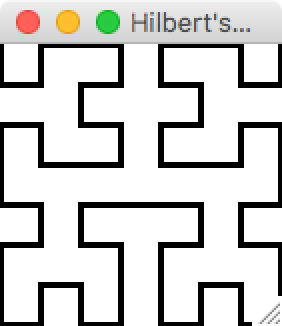
\includegraphics[width=0.45\textwidth]{hilbert3}
  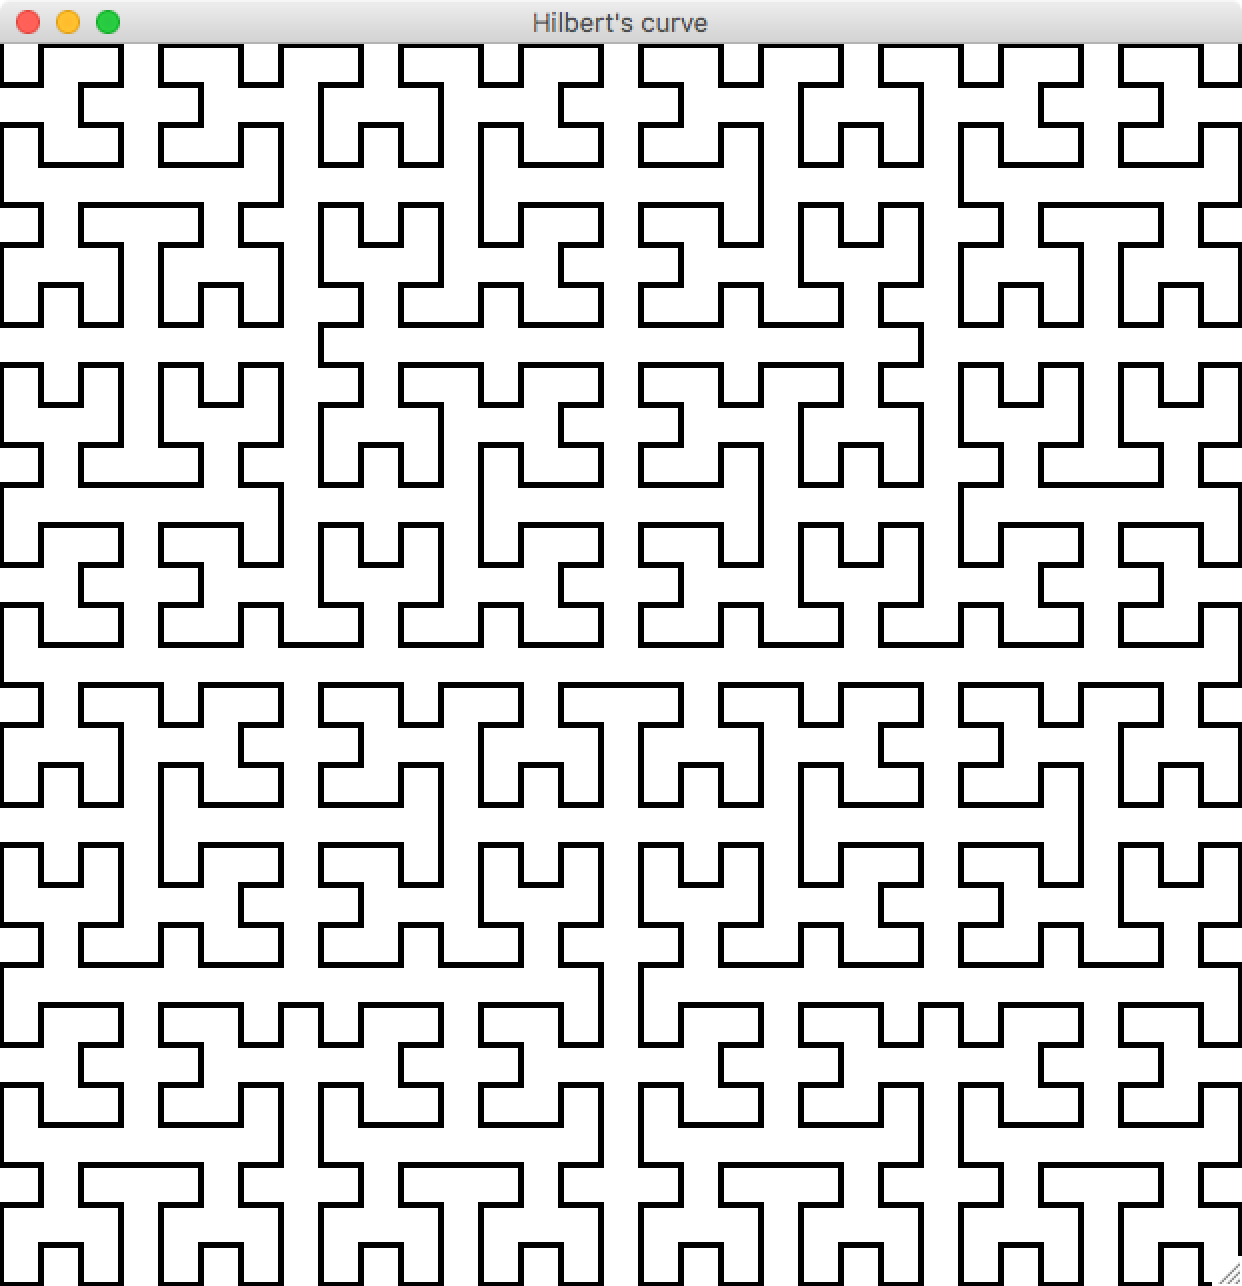
\includegraphics[width=0.45\textwidth]{hilbert5}
  \caption{Hilbert curves of order 1, 2, 3, and 5 by code in Listing~\ref{winforms/hilbert}.}
  \label{fig:hilbert1}
\end{figure}

%
\fsCode{winforms/windowEvents}{Catching window, mouse, and keyboard events..}
%

\section{Buttons and stuff}

%
\fsCode{winforms/buttonControl}{Create the button and an event.}
%
\begin{figure}
  \centering
  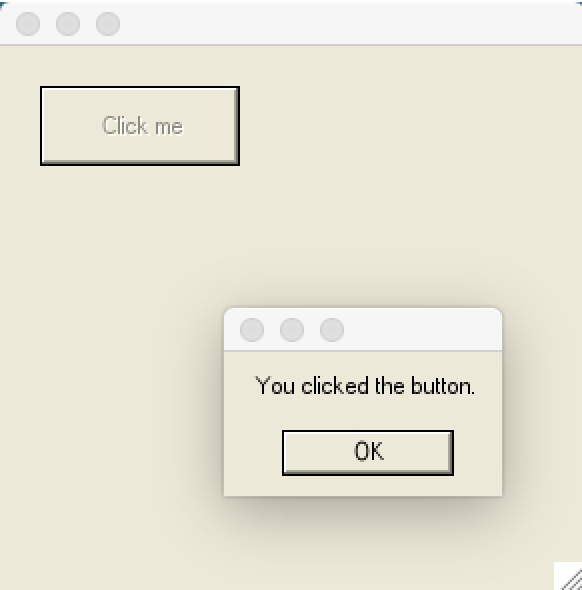
\includegraphics[width=0.6\textwidth]{buttonControl}
  \caption{A button is pressed and the event handler calls the \lstinline!MessageBox.Show! dialogue window by the code in Listing~\ref{winforms/buttonControl}.}
  \label{fig:buttonControl}
\end{figure}

%
\fsCode{winforms/panel}{Create a panel, label, text input controls.}
%
\begin{figure}
  \centering
  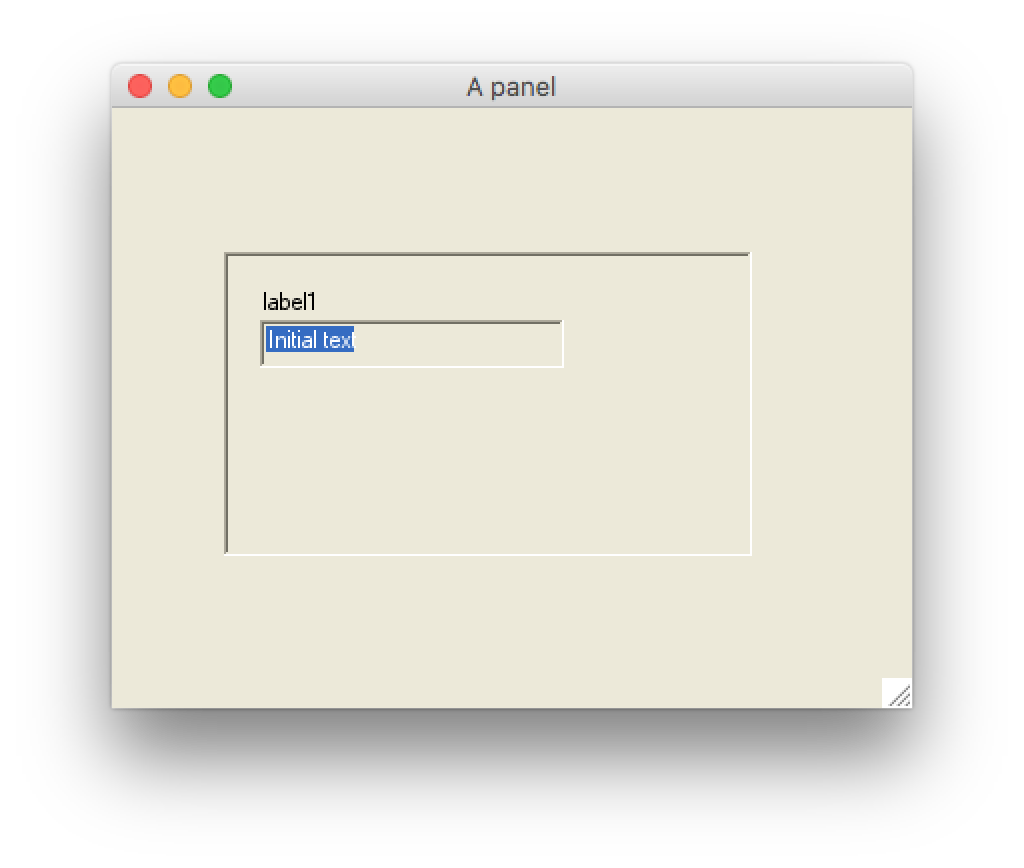
\includegraphics[width=0.6\textwidth]{panel}
  \caption{A panel including a label and a text input field, see Listing~\ref{winforms/panel}.}
  \label{fig:panel}
\end{figure}

%
\fsCode[lastline=42]{winforms/flowLayoutPanel}{Create a flowLayoutPanel, with checkbox and radiobuttons.}
%
%
\fsCode[firstnumber=43,firstline=43,lastline=87]{winforms/flowLayoutPanel}{Create a flowLayoutPanel, with checkbox and radiobuttons.}
%
%
\fsCode[firstnumber=88,firstline=88]{winforms/flowLayoutPanel}{Create a flowLayoutPanel, with checkbox and radiobuttons.}
%
\begin{figure}
  \centering
  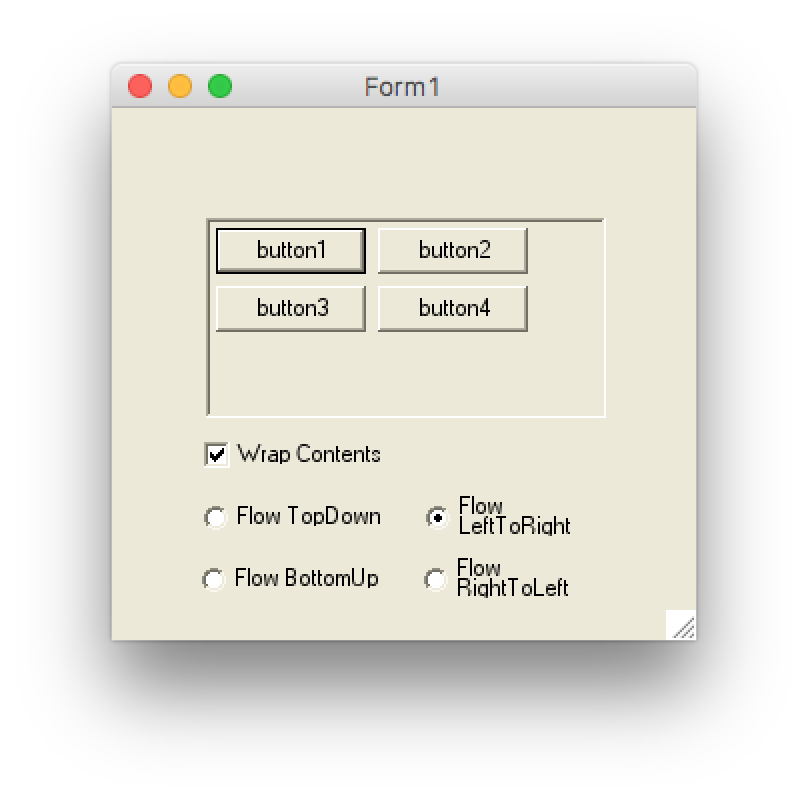
\includegraphics[width=0.6\textwidth]{flowLayoutPanel}
  \caption{Demonstration of the \lstinline!FlowLayoutPanel! panel, \lstinline!CheckBox!, and \lstinline!RadioButton! controls, see Listing~\ref{winforms/flowLayoutPanel}.}
  \label{fig:flowLayoutPanel}
\end{figure}



\jon{\lstinline!Click.Add! expects a function \lstinline!System.EventArgs -> unit! therfore the \lstinline!ignore! function.}

\begin{table}
  \begin{center}
  \rowcolors{2}{oddRowColor}{evenRowColor}
    \begin{tabularx}{\linewidth}{|l|X|}
      \hline
      \rowcolor{headerRowColor}  Function & Description\\
      \hline
      \lstinline{DataGridView}
      &Display data on a table.\\
      \hline
      \lstinline{TextBox}
      &Display editable text.\\
      \hline
      \lstinline{Label}
      &Display text.\\
      \hline
      \lstinline{LinkLabel}
      &Display clickable text.\\
      \hline
      \lstinline{ProgressBar}
      &Display the current progress as a bar.\\
      \hline
      \lstinline{WebBrwoser}
      &Enable navigation of the web.\\
      \hline
      \lstinline{CheckedListBox}
      &Display a scrollable check box list.\\
      \hline
      \lstinline{ComboBox}
      &Display a drop-down list.\\
      \hline
      \lstinline{ListBox}
      &Display a list of text and icons.\\
      \hline
      \lstinline{PictureBox}
      &Display a bitmap image\\
      \hline
      \lstinline{CheckBox}
      &Display a checkbox and a label of text.\\
      \hline
      \lstinline{RadioButton}
      &Display an on-off radio button\\
      \hline
      \lstinline{TrackBar}
      &Enable the user to input value by moving a cursor on a slider bar\\
      \hline
      \lstinline{DateTimePicker}
      &Enable the user to select a date from a graphical calendar\\
      \hline
      \lstinline{ColorDialogue}
      &Enable the user to pick a color\\
      \hline
      \lstinline{FontDialog}
      &Enable the user to pick a font and its attributes\\
      \hline
      \lstinline{OpenFileDialog}
      &Enable the user to navigate the file system and select a file..\\
      \hline
      \lstinline{PrintDialog}
      &Enable the user to select a printer and its attributes.\\
      \hline
      \lstinline{SaveDialog}
      &Enable the user to navigate the file system and specify a filename.\\
      \hline
      \lstinline{MenuStrip}
      &Allow the user to choose from a custom menu\\
      \hline
      \lstinline{Button}
      &Display a clickable button with text\\
      \hline
      \lstinline{Tooltip}
      &Briefly display a pop-up window, when the user rests the pointer on the control\\
      \hline
      \lstinline{SoundPlayer}
      &Play sounds in the \lstinline{.wav} format.\\
      \hline
    \end{tabularx}
  \end{center}
  \caption{Some controls available in WinForms.}
  \label{tab:controls}
\end{table}

\begin{table}
  \begin{center}
  \rowcolors{2}{oddRowColor}{evenRowColor}
    \begin{tabularx}{\linewidth}{|l|X|}
      \hline
      \rowcolor{headerRowColor}  Function & Description\\
      \hline
      \lstinline{Panel}
      &Groups a set of controls in a scrollable frame.\\
      \hline
      \lstinline{GroupBox}
      &Group a set of controls in a non-scrollable frame.\\
      \hline
      \lstinline{TabControl}
      &Group controls in tabpages, A tabpage is selected by clicking on its tab.\\
      \hline
      \lstinline{SplitContainer}
      &Group controls into two resizable panels.\\
      \hline
      \lstinline{TableLayoutPanel}
      &Group controls into a grid.\\
      \hline
      \lstinline{FlowLayoutPanel}
      &Group controls into a set of flowable panels. The panels may flow horizontally or vertically as a response to window resizing.\\
      \hline
    \end{tabularx}
  \end{center}
  \caption{Some controls for grouping other controls.}
  \label{tab:controlGroups}
\end{table}

\dots

%%% Local Variables:
%%% TeX-master: "fsharpNotes"
%%% End:
